\documentclass[../main.tex]{subfiles}

\begin{document}
\section{Task 1 -- XGBoost}
The model was trained using mostly default parameters of the Python
\verb`xgboost` module. Despite this, it managed to achieve quite tremendous
results, as visible in table \ref{table:perf}.

\subsection{Model visualization}
\begin{figure}[H]
	\centering
	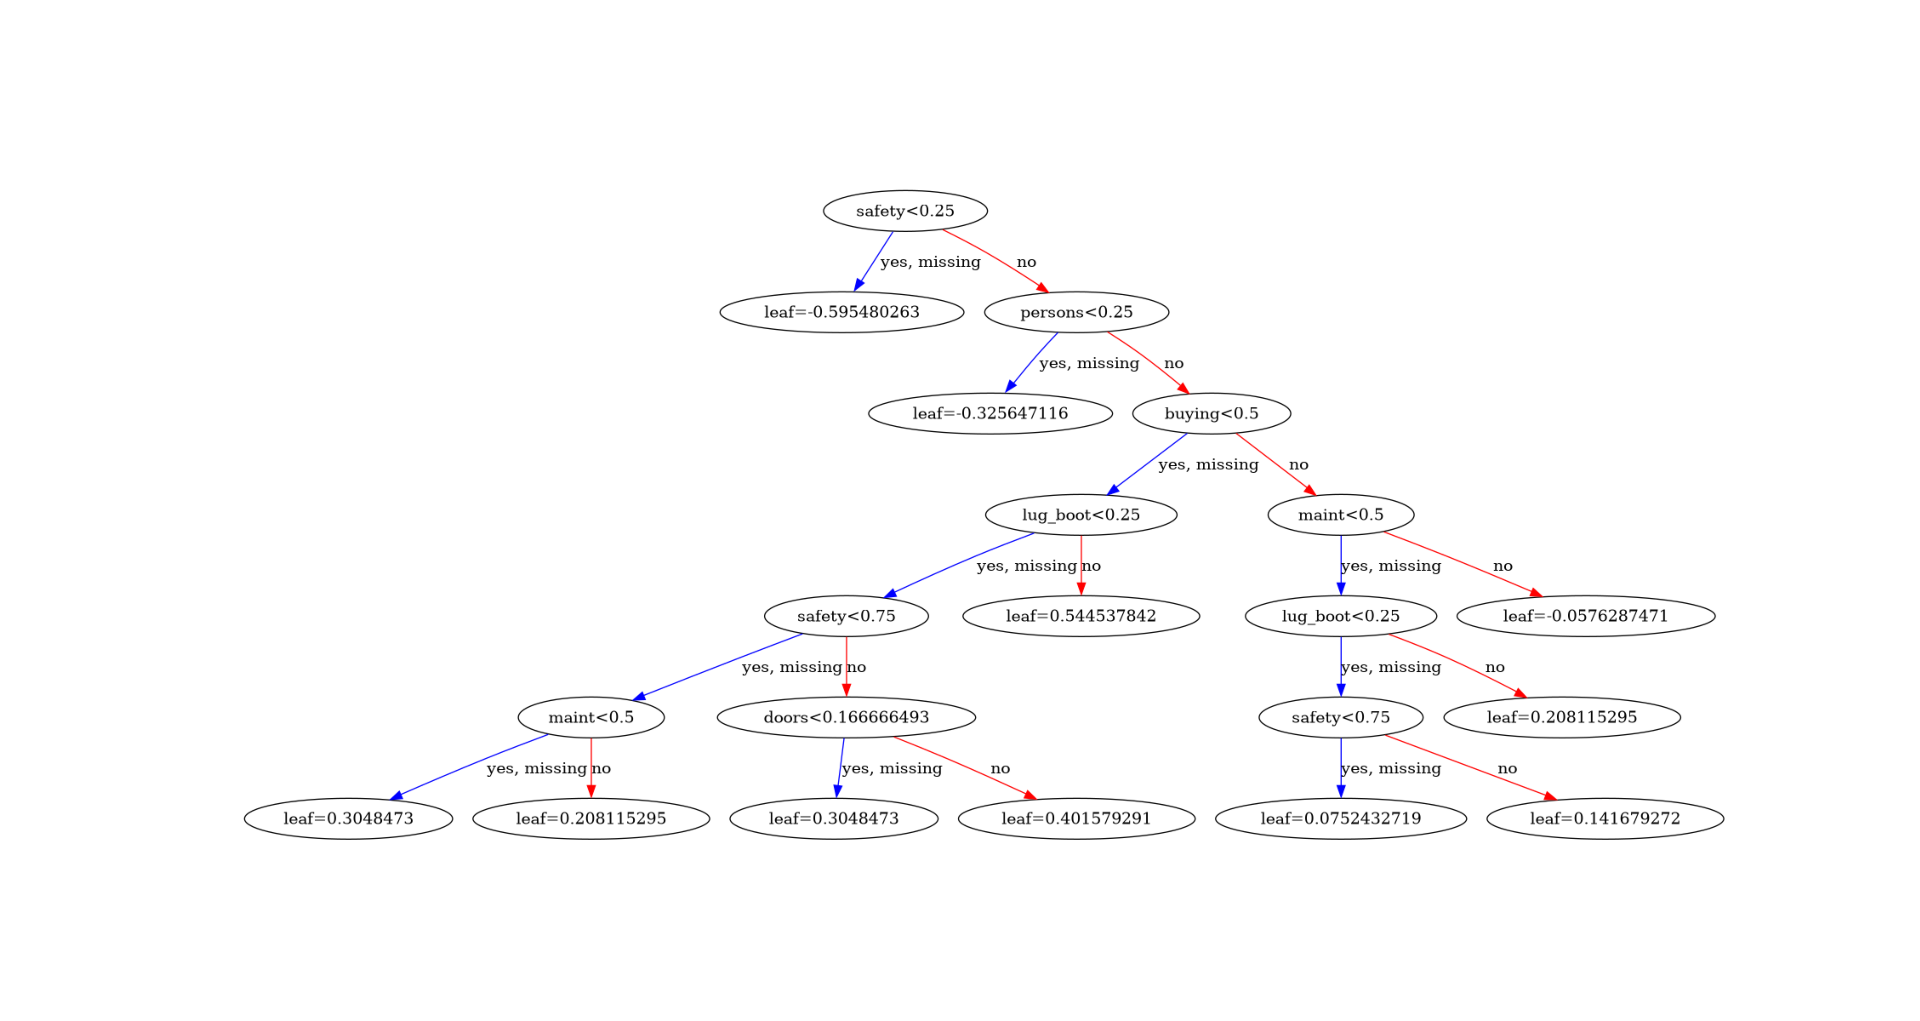
\includegraphics[width=\linewidth]{../img/xgb-tree.png}
	\caption{Last tree in the ensemble produced by XGBoost}
	\label{fig:xgb-tree}
\end{figure}

\subsection{Preference analysis}
\begin{figure}[H]
	\centering
	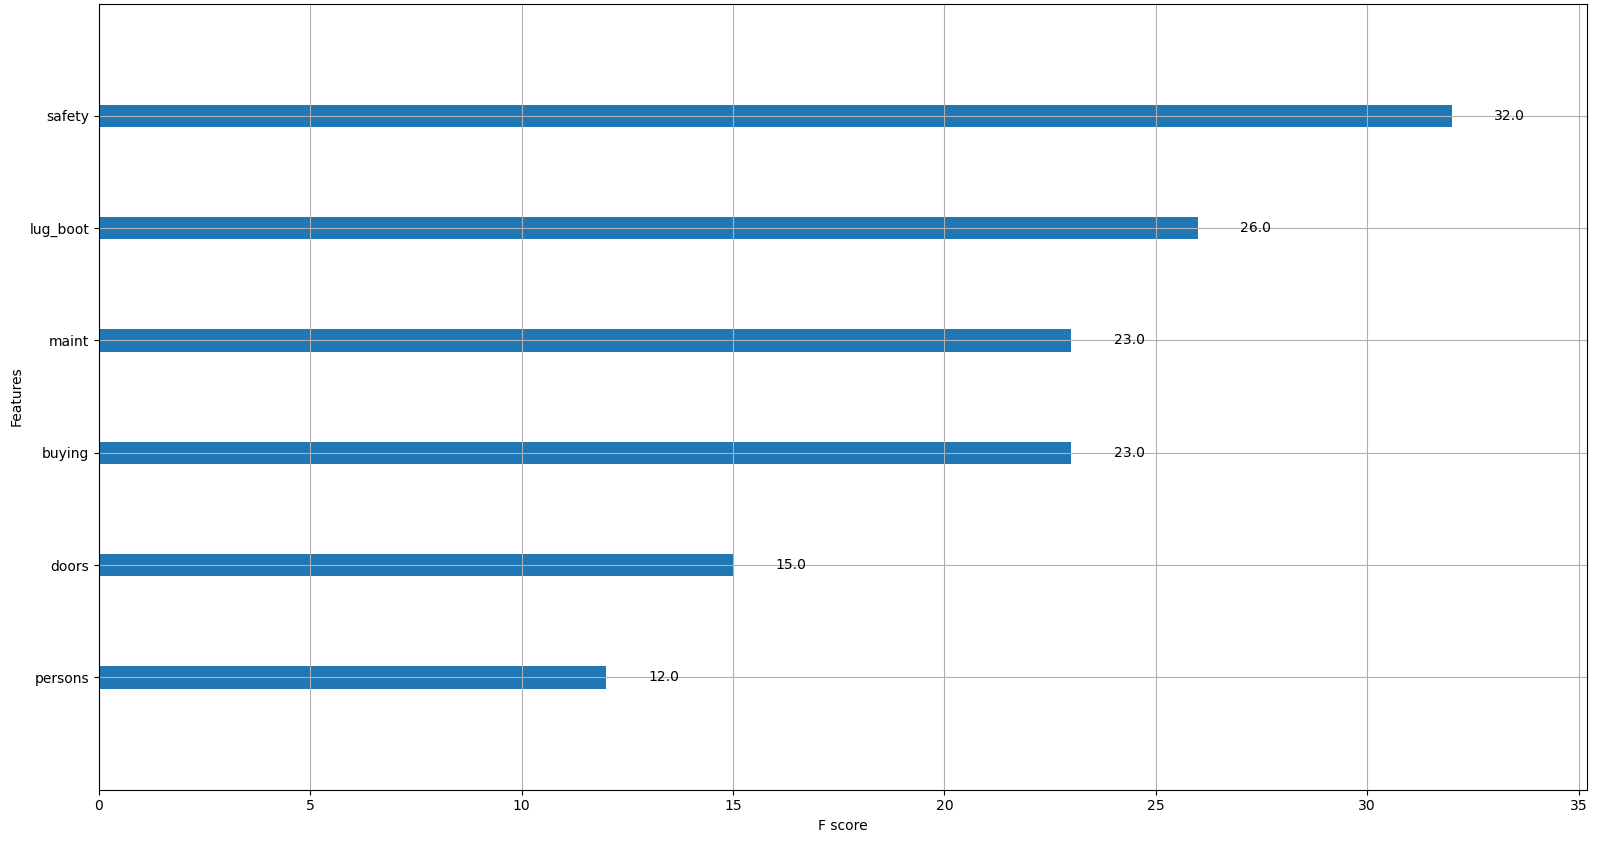
\includegraphics[width=\linewidth]{../img/xgb-feature-importance.png}
	\caption{XGBoost feature importance as computed by DALEX}
	\label{fig:xgb-feats}
\end{figure}
DALEX assigns very high importance to \emph{persons} and \emph{safety}, in that
order. This aligns with figure \ref{fig:xgb-3alt-allcetpar} of the forthcoming
ceteris paribus analysis. These importances don't fully agree with the above
model visualization (in which \emph{safety} seems to play a more significant
role), but it is important to keep in mind that the visualization is merely of
a single tree in an ensemble.

\paragraph{XGBoost} The XGBoost library also has native support for quantifying
and plotting feature importance. It must use a slightly different method than
DALEX, because the assigned values and even the ranking of the features are not
the same. For the sake of inter-model comparability, we prioritized the DALEX
output, but nevertheless this interpretation is also interesting:
\begin{figure}[H]
	\centering
	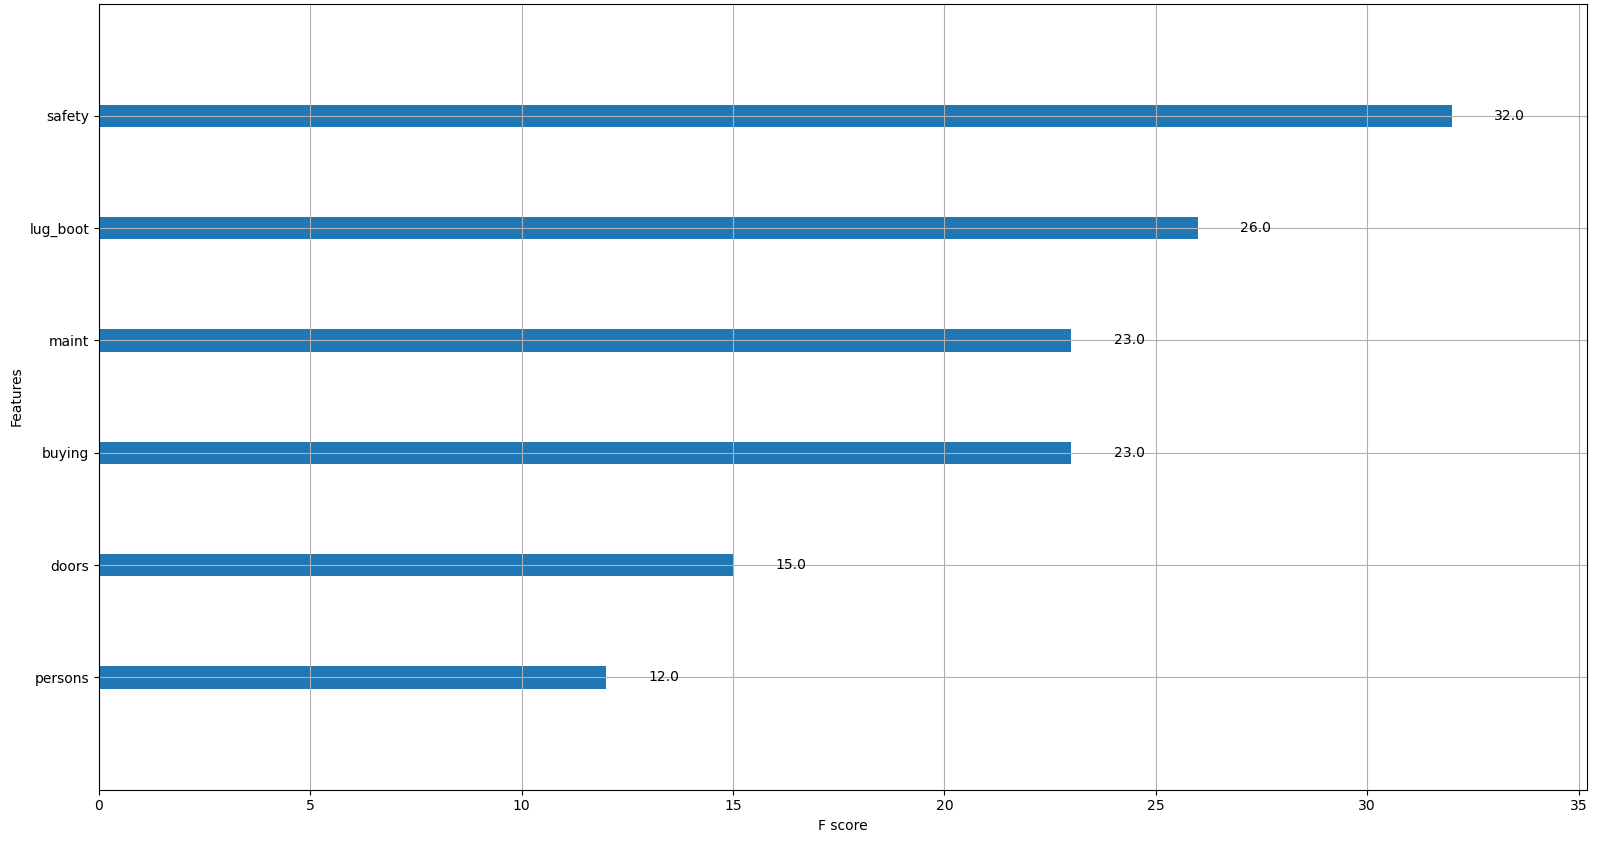
\includegraphics[width=\linewidth]{../img/xgb-feature-importance-xgboost.png}
	\caption{Importance of each feature, according to XGBoost}
	\label{fig:xgb-feats-xgboost}
\end{figure}
What is quite frankly shocking is the assignment of the lowest importance score
to \emph{persons}. This runs counter to both our intuitive expectations and
other analyses.

\subsection{3-alternative analysis}
\subsubsection{Analytical approach}
Predicting the outcome of a tree ensemble method is certainly not as trivial as
doing so with only a single tree. However, for the sake of simplicity, I will
assume that a single tree is a sufficiently accurate approximation of the
entire model and make judgements based on the final tree in the ensemble
produced by XGBoost, as seen on figure \ref{fig:xgb-tree}.
\paragraph{Alternative 1} This alternative has 0 \emph{safety}, which
disqualifies it on the very first tree branch (we want a positive leaf value).
Following the model's parameters, it would need a \emph{safety} of at least
\verb`0.25`. Using the same logic for subsequent branches, \emph{persons} would
need to be at least \verb`0.25` as well. From there the tree becomes more
complex, so I will assume a simple greedy strategy and only tweak feature
values when absolutely necessary. We proceed to the right with \emph{buying}
unchanged. Then we must lower \emph{maint} by more than \verb`0.5`. After
that, all leaves are positive, so there is no need for further changes.
% TODO

\subsubsection{Space sampling}
Most plots were approximately "flat", with no major shifts in prediction
(Y-axis). What this generally means is that those features alone can't swivel
the classification of an alternative.

There are, however, 2 features that do exhibit some major shifts --
\emph{safety} and \emph{persons}:
\begin{figure}[H]
	\centering
	\begin{subfigure}[b]{0.32\linewidth}
		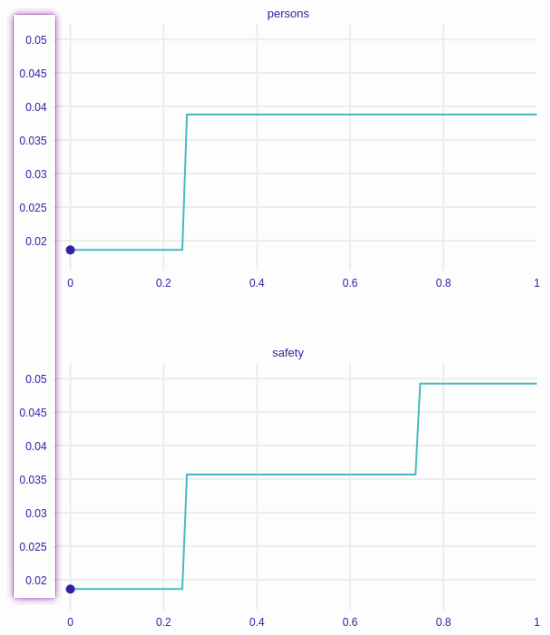
\includegraphics[width=\linewidth]{../img/xgb-cetpar-worst.png}
		\caption{alternative 1 (worst)}
		\label{fig:xgb-3alt1-cetpar}
	\end{subfigure}
	\begin{subfigure}[b]{0.32\linewidth}
		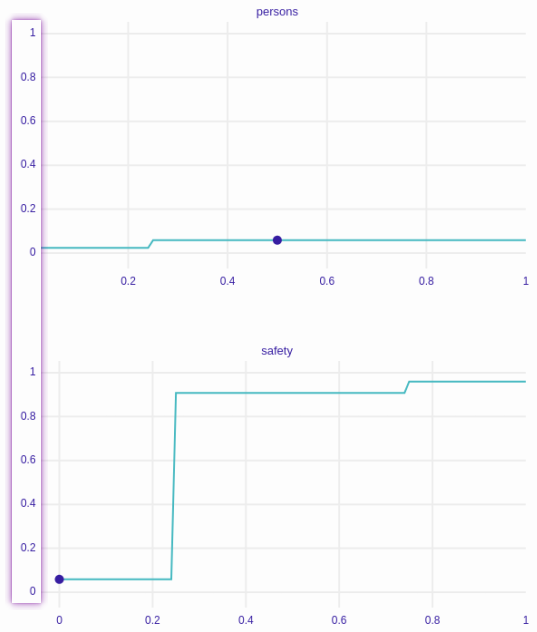
\includegraphics[width=\linewidth]{../img/xgb-cetpar-mid.png}
		\caption{alternative 2 (mid)}
		\label{fig:xgb-3alt1-cetpar}
	\end{subfigure}
	\begin{subfigure}[b]{0.32\linewidth}
		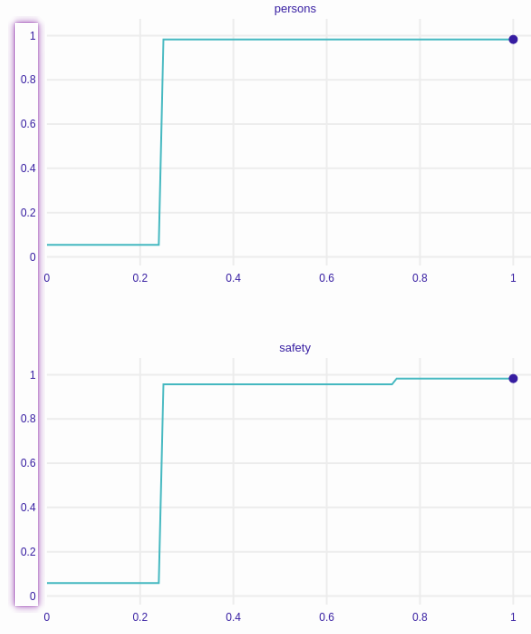
\includegraphics[width=\linewidth]{../img/xgb-cetpar-best.png}
		\caption{alternative 3 (best)}
		\label{fig:xgb-3alt1-cetpar}
	\end{subfigure}
	\caption{Ceteris paribus of \emph{persons} and \emph{safety} features in XGBoost}
	\label{fig:xgb-3alt-allcetpar}
\end{figure}
For alternative 2, \emph{safety} is very highly correlated with the decision
class. There is a clear boundary at around \verb`0.25` where the model leaps
from being barely above 0 to being almost 1. This suggests that there were many
middle alternatives which were unacceptable solely due to a low \emph{safety}
value. The same observation can be made for alternative 3 and both
\emph{persons} and \emph{safety}.

A bonus observation is that these plots resemble \textbf{step functions}. That
is because XGBoost is a tree ensemble model, and trees are unable to produce
smooth decision boundaries due to their nature of branching on specific feature
values.

\subsubsection{Variable contribution plots}
\begin{figure}[H]
	\centering
	\begin{subfigure}{\linewidth}
		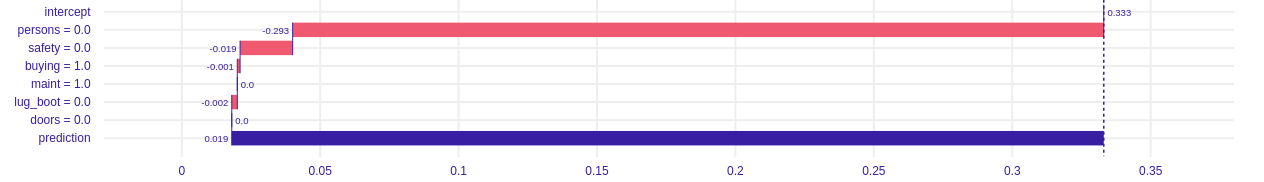
\includegraphics[width=\linewidth]{../img/xgb-breakdown-worst.png}
		\caption{Variable contribution of alternative 1 (worst) in XGBoost}
		\label{fig:xgb-3alt1-contrib}
	\end{subfigure}
	\begin{subfigure}{\linewidth}
		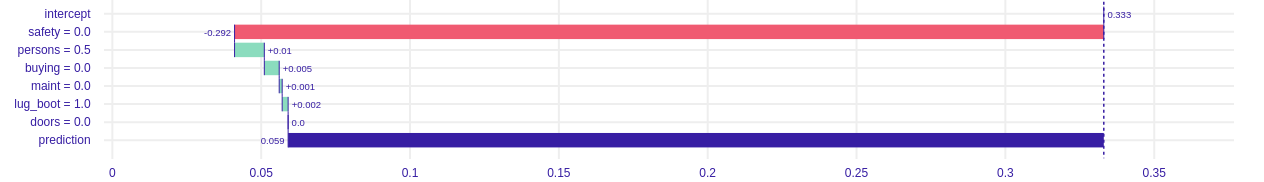
\includegraphics[width=\linewidth]{../img/xgb-breakdown-mid.png}
		\caption{Variable contribution of alternative 2 (mid) in XGBoost}
		\label{fig:xgb-3alt2-contrib}
	\end{subfigure}
	\begin{subfigure}{\linewidth}
		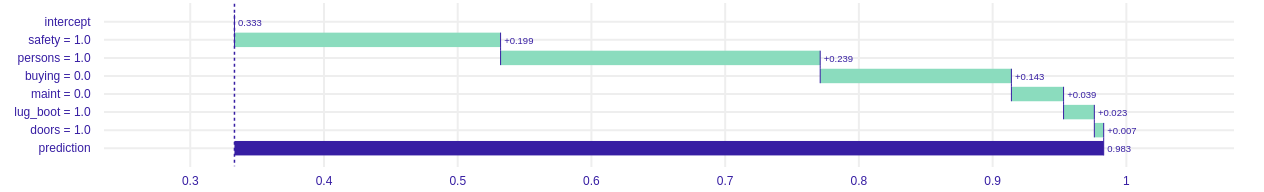
\includegraphics[width=\linewidth]{../img/xgb-breakdown-best.png}
		\caption{Variable contribution of alternative 3 (best) in XGBoost}
		\label{fig:xgb-3alt3-contrib}
	\end{subfigure}
\end{figure}
% TODO interpret
\end{document}
